\subsection{Opgave 24}

På figuren nedenfor ses repræsentanter for vektorerne $\vec{a}$, $\vec{b}$ og $\vec{c}$.

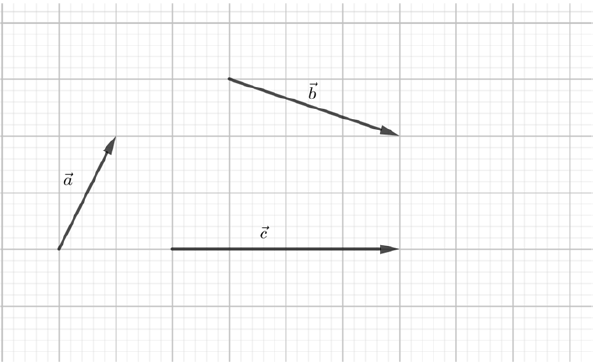
\includegraphics[width = 0.5\textwidth]{Opgave_21-30/Opgave_24/24.png}

Indtegn en repræsentant for vektoren $\vec{a} + \vec{b} + \vec{c}$.

\ans

Først aflæser vi vektorernes x og y komponenter. X komponenten af en vektor er hvor meget vi går hen ad x - aksen, og y komponent er hvor meget vi går op ad y aksen. Nedenstående figur illustrerer hvordan man kan aflæse en vektors x og y komponenter ud fra figuren. 

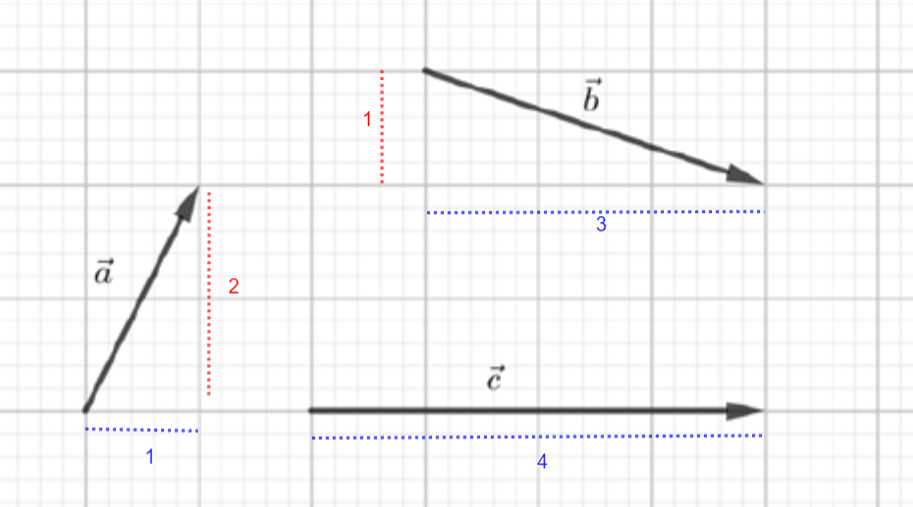
\includegraphics[width = 0.5\textwidth]{Opgave_21-30/Opgave_24/24.1.png}

De blå linjer er vektorernes x komponenter og de røde linjer er vektorernes y komponenter.

Vi har nu
\begin{align*}
    \Vec{a} &= \begin{pmatrix} 1 \\ 2 \end{pmatrix}\\
    \Vec{b} &= \begin{pmatrix} 3 \\ -1 \end{pmatrix}\\
    \Vec{c} &= \begin{pmatrix} 4 \\ 0 \end{pmatrix}
\end{align*}

Vi kan nu beregne summen af de 3 vektorer
\begin{align*}
    \Vec{a} + \Vec{b} + \Vec{c} = \begin{pmatrix} 1 \\ 2 \end{pmatrix} + \begin{pmatrix} 3 \\ -1 \end{pmatrix} + \begin{pmatrix} 4 \\ 0 \end{pmatrix} = \begin{pmatrix}
        1 + 3 + 4 \\ 2 - 1 + 0
    \end{pmatrix}  = \begin{pmatrix}
        8 \\ 1
    \end{pmatrix}
\end{align*}

Nu indtegner vi vektoren $\begin{pmatrix}
    8 \\ 1
\end{pmatrix}$
ind i et koordinatsystem. 

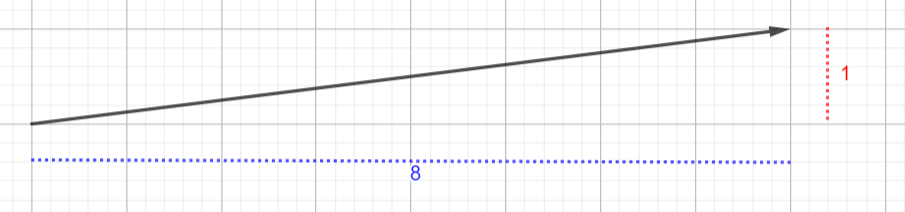
\includegraphics[width = 0.5\textwidth]{Opgave_21-30/Opgave_24/24.2.png}